\chapter{Aprendizaje Profundo para Clasificación de Gestos}
\label{cp:aprendizaje-profundo}

\insertminitoc
\parindent0pt

El reconocimiento automático de señas exige transformar secuencias de coordenadas
corporales en etiquetas lingüísticas. Los capítulos anteriores describieron cómo
MediaPipe Hands extrae 21 puntos de referencia tridimensionales por mano detectada
\cite{zhang_mediapipe_2020}, \cite{bazarevsky_blazepalm_2019},
\cite{lugaresi_mediapipe_2019}. El presente capítulo aborda los modelos de aprendizaje
profundo que reciben esos vectores de landmarks y producen la clasificación final de
la seña, así como las técnicas que permiten ejecutar dichos modelos localmente en el
dispositivo móvil sin conexión a internet.

\section{Fundamentos de las Redes Neuronales Artificiales}

Una red neuronal artificial está compuesta por unidades de cómputo llamadas neuronas.
Cada neurona recibe un vector de entradas, lo multiplica por pesos sinápticos, suma un
término de sesgo y aplica una función de activación no lineal para producir su salida.
Rosenblatt formalizó este modelo en 1958 bajo el nombre de perceptrón
\cite{rosenblatt_perceptron_1958}. En su forma original, el perceptrón solo podía
resolver problemas linealmente separables, limitación que se superó al apilar varias
capas de neuronas y entrenarlas con el algoritmo de retropropagación del error,
desarrollado por Rumelhart, Hinton y Williams en 1986 \cite{rumelhart_backprop_1986}.
Este algoritmo calcula el gradiente de una función de pérdida respecto a cada peso de
la red mediante la regla de la cadena, y actualiza los parámetros en la dirección que
reduce el error.

Las redes con múltiples capas ocultas, conocidas como redes profundas, aprenden
representaciones jerárquicas de los datos \cite{goodfellow_deep_2016},
\cite{lecun_deep_2015}. En problemas de clasificación multiclase, la función de pérdida
estándar es la entropía cruzada categórica, y la capa de salida utiliza la función
softmax para convertir los logits en una distribución de probabilidad sobre las clases.
El optimizador Adam, propuesto por Kingma y Ba en 2015, adapta la tasa de aprendizaje
de cada parámetro de forma individual a partir de estimaciones del primer y segundo
momento de los gradientes, lo que acelera la convergencia en conjuntos de datos con
gradientes ruidosos \cite{kingma_adam_2015}. Para prevenir el sobreajuste, se aplica
dropout durante el entrenamiento, técnica que desactiva aleatoriamente neuronas con una
probabilidad fija y obliga a la red a distribuir la representación aprendida entre
múltiples unidades \cite{srivastava_dropout_2014}.

La \autoref{fig:teoria-neurona} resume estos elementos: la unidad básica de cálculo y la
forma en que se organiza al apilarse en capas.

\begin{figure}[htbp]
\centering
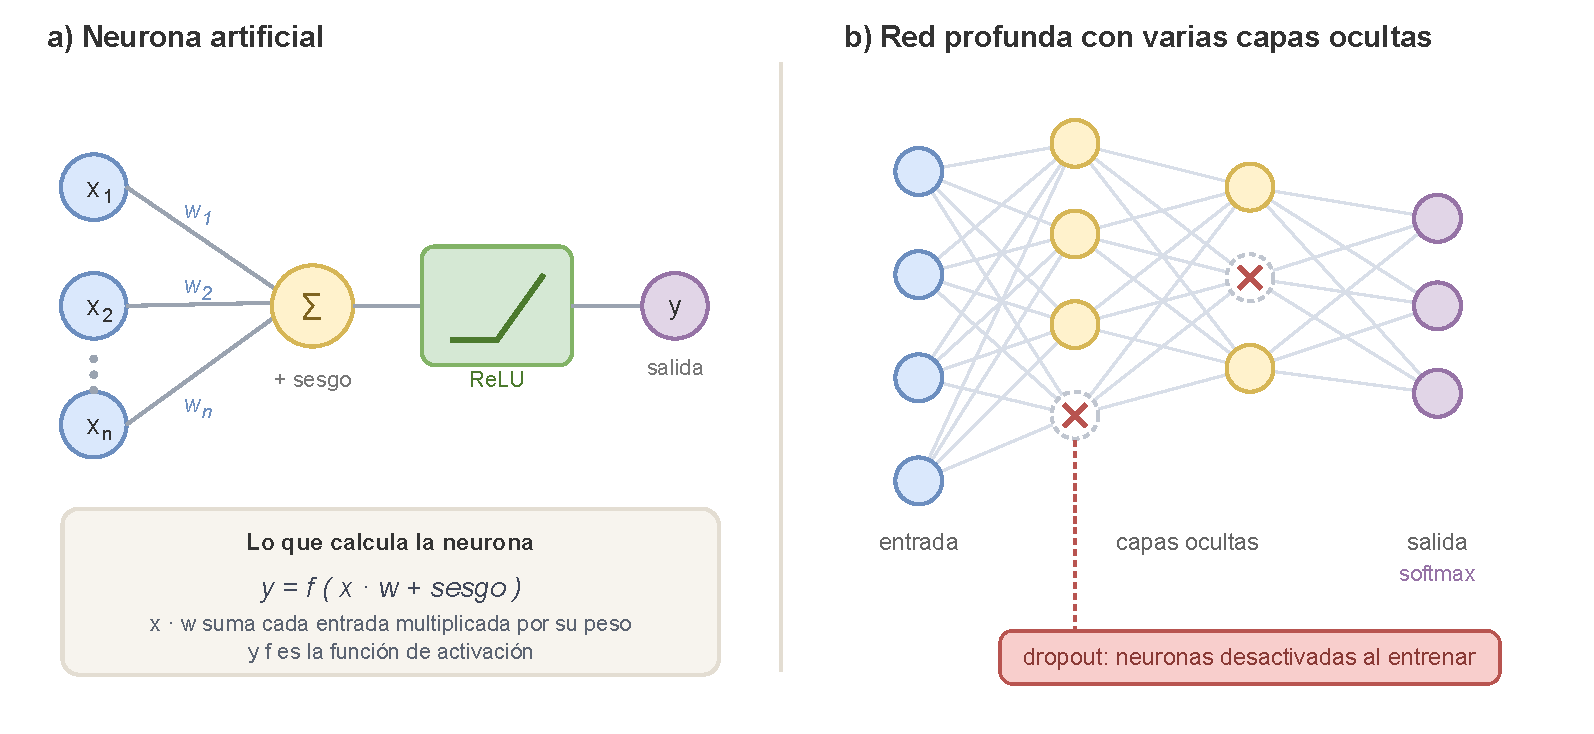
\includegraphics[width=\textwidth]{Figures/Teoria/neurona_red.pdf}
\caption[Neurona artificial y red profunda]{Neurona artificial y red profunda. A la
izquierda, la unidad de cálculo: las entradas se ponderan, se suman junto con el sesgo y
el resultado pasa por una función de activación. A la derecha, la organización en capas,
con la salida softmax y las neuronas que el dropout desactiva durante el entrenamiento.
Fuente: Elaboración propia.}
\label{fig:teoria-neurona}
\end{figure}

Conviene observar en la \autoref{fig:teoria-neurona} que el dropout no elimina neuronas
del modelo: solo las
desactiva de forma temporal y aleatoria en cada paso del entrenamiento, lo que impide que
la red dependa en exceso de unas pocas unidades. En la inferencia, todas vuelven a
participar.

\section{Red Convolucional 1D para la Clasificación del Alfabeto}

El módulo de reconocimiento del alfabeto dactilológico no clasifica un único fotograma,
sino una ventana temporal corta de los últimos 20 fotogramas. Cada fotograma se
representa con un vector de 126 valores, que corresponde a 21 landmarks por mano con
coordenadas $x$, $y$, $z$ para las dos manos. La salida es una de las 33 clases del
sistema: las 30 letras del alfabeto dactilológico del \acrshort{lesho}, incluidos los dígrafos
CH, LL y RR, la clase REPOSO y dos señas de control.

La razón de clasificar una ventana y no un solo fotograma es que cinco letras del
alfabeto, la J, la Ñ, la Z, la LL y la RR, se ejecutan con movimiento, por lo que una
sola pose no las representa. Una ventana de fotogramas captura la trayectoria completa
de estas letras, mientras que una letra estática produce una ventana en la que todos los
fotogramas son casi idénticos. De este modo, una misma arquitectura reconoce tanto las
letras estáticas como las que llevan movimiento.

Para esta tarea se emplea una red neuronal convolucional en una dimensión (\acrshort{cnn} 1D).
Una convolución aplica un filtro que se desliza a lo largo de un eje, en este caso el eje
temporal de la ventana, y detecta patrones locales, como el cambio de forma de la mano
entre fotogramas consecutivos. La red aprende múltiples filtros de este tipo y combina
sus salidas para clasificar la ventana. Frente a una red recurrente, la convolución en
una dimensión es más ligera, se ejecuta de forma paralela y se convierte al formato de
inferencia móvil sin operaciones especiales, lo que la hace idónea para la ejecución en
tiempo real en el dispositivo \cite{goodfellow_deep_2016}, \cite{lecun_deep_2015}.

Antes de alimentar la red, los landmarks de cada fotograma se normalizan en dos pasos.
Primero se resta la coordenada de la muñeca a todos los demás puntos de la misma mano,
de modo que la mano queda centrada en el origen con independencia de su posición en el
encuadre. Luego se divide por el tamaño de la mano, lo que elimina la variación por
distancia de la mano a la cámara. Con esta normalización, la red aprende la configuración
geométrica de la seña y no su posición o escala absoluta en la imagen
\cite{zhang_mediapipe_2020}. El modelo se compone de bloques convolucionales con
activación \acrshort{relu} y agrupación temporal, seguidos de una capa densa con
regularización dropout y una capa de salida softmax de 33 neuronas.

La \autoref{fig:teoria-convolucion} ilustra este funcionamiento sobre la ventana temporal,
junto con la normalización previa de los landmarks.

\begin{figure}[htbp]
\centering
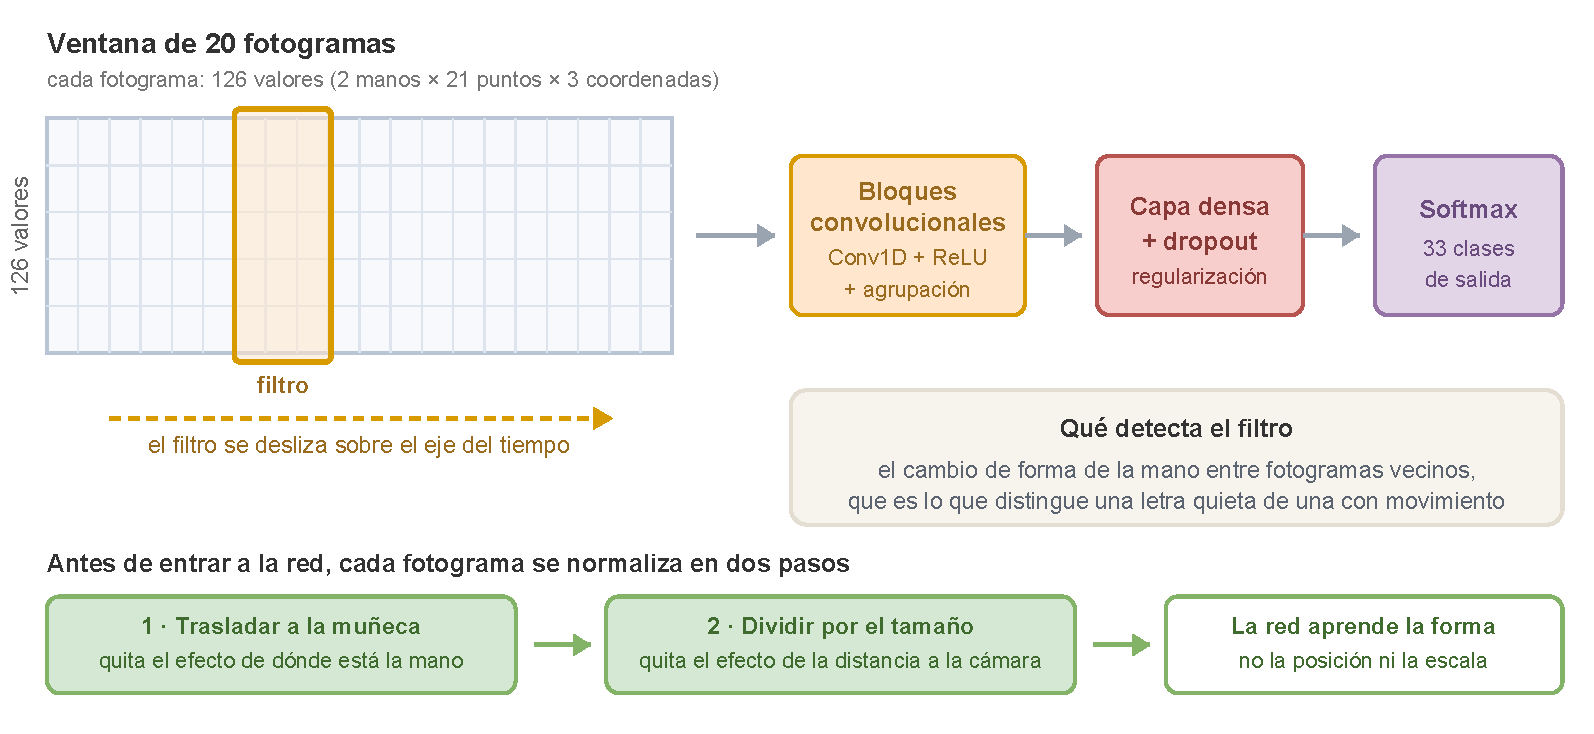
\includegraphics[width=\textwidth]{Figures/Teoria/convolucion_1d.pdf}
\caption[Convolución en una dimensión sobre la ventana temporal]{Convolución en una
dimensión sobre la ventana temporal. El filtro recorre el eje del tiempo y detecta
patrones locales entre fotogramas vecinos; abajo se muestran los dos pasos de
normalización que se aplican a cada fotograma antes de entrar a la red. Fuente:
Elaboración propia.}
\label{fig:teoria-convolucion}
\end{figure}

El detalle que explica la elección de esta arquitectura está en el eje sobre el que se
desliza el filtro. Al recorrer el tiempo y no el espacio de la imagen, la red no compara
formas de mano aisladas sino su evolución entre fotogramas consecutivos, que es
precisamente la información que separa una letra sostenida de una que se ejecuta con
movimiento.

\section{Redes Recurrentes (LSTM y GRU) para Clasificación de Secuencias}

Las señas dinámicas de \acrshort{lesho} involucran movimiento: la mano recorre una trayectoria
en el espacio durante un intervalo de tiempo que puede abarcar varios segundos. A
diferencia de la ventana corta del alfabeto, una seña completa exige modelar dependencias
temporales de mayor alcance, para lo cual conviene una arquitectura con memoria explícita.
Las redes neuronales recurrentes
(\acrshort{rnn}) abordan este problema mediante conexiones cíclicas: la salida en el paso temporal
$t$ depende tanto de la entrada actual como del estado oculto previo, que resume la
información de todos los pasos anteriores. Sin embargo, las \acrshort{rnn} simples sufren el
problema del desvanecimiento del gradiente en secuencias largas, que impide aprender
dependencias a largo plazo \cite{goodfellow_deep_2016}.

La arquitectura Long Short-Term Memory (\acrshort{lstm}), propuesta por Hochreiter y Schmidhuber
en 1997, resuelve este problema mediante tres compuertas multiplicativas
\cite{hochreiter_lstm_1997}. La compuerta de olvido decide qué información del estado
de celda anterior se descarta; la compuerta de entrada controla qué nueva información
se almacena; y la compuerta de salida determina qué parte del estado de celda se expone
como estado oculto. La compuerta de olvido, incorporada por Gers, Schmidhuber y Cummins
en 2000, resulta especialmente relevante para procesar flujos continuos de landmarks de
video \cite{gers_forget_2000}. La unidad recurrente con compuertas (\acrshort{gru}), propuesta por
Cho et al. en 2014, simplifica la arquitectura \acrshort{lstm} al reducir las tres compuertas a
dos, lo que disminuye el número de parámetros sin pérdida significativa de rendimiento
en muchas tareas de secuencias \cite{cho_gru_2014}. Para la clasificación de las 50
señas dinámicas del sistema, se emplea una red \acrshort{lstm} en configuración many-to-one: la
red procesa la secuencia completa de cuadros capturados durante la grabación y
emite una única clasificación al final, tomando el estado oculto del último paso temporal
como entrada a una capa densa de salida softmax. Esta elección se sustenta en la
capacidad demostrada de la \acrshort{lstm} para clasificar secuencias de landmarks de manos en
trabajos previos sobre reconocimiento de lenguas de señas \cite{mittal_lstm_2019},
\cite{khartheesvar_indian_2024}, y en una razón práctica de despliegue: la \acrshort{lstm} cuenta
con una operación fusionada en el marco de inferencia móvil que permite ejecutarla de
forma eficiente en el dispositivo, optimización de la que la \acrshort{gru} no dispone.

La \autoref{fig:teoria-lstm} compara ambas celdas y resume el criterio con que se eligió
una de las dos para este sistema.

\begin{figure}[htbp]
\centering
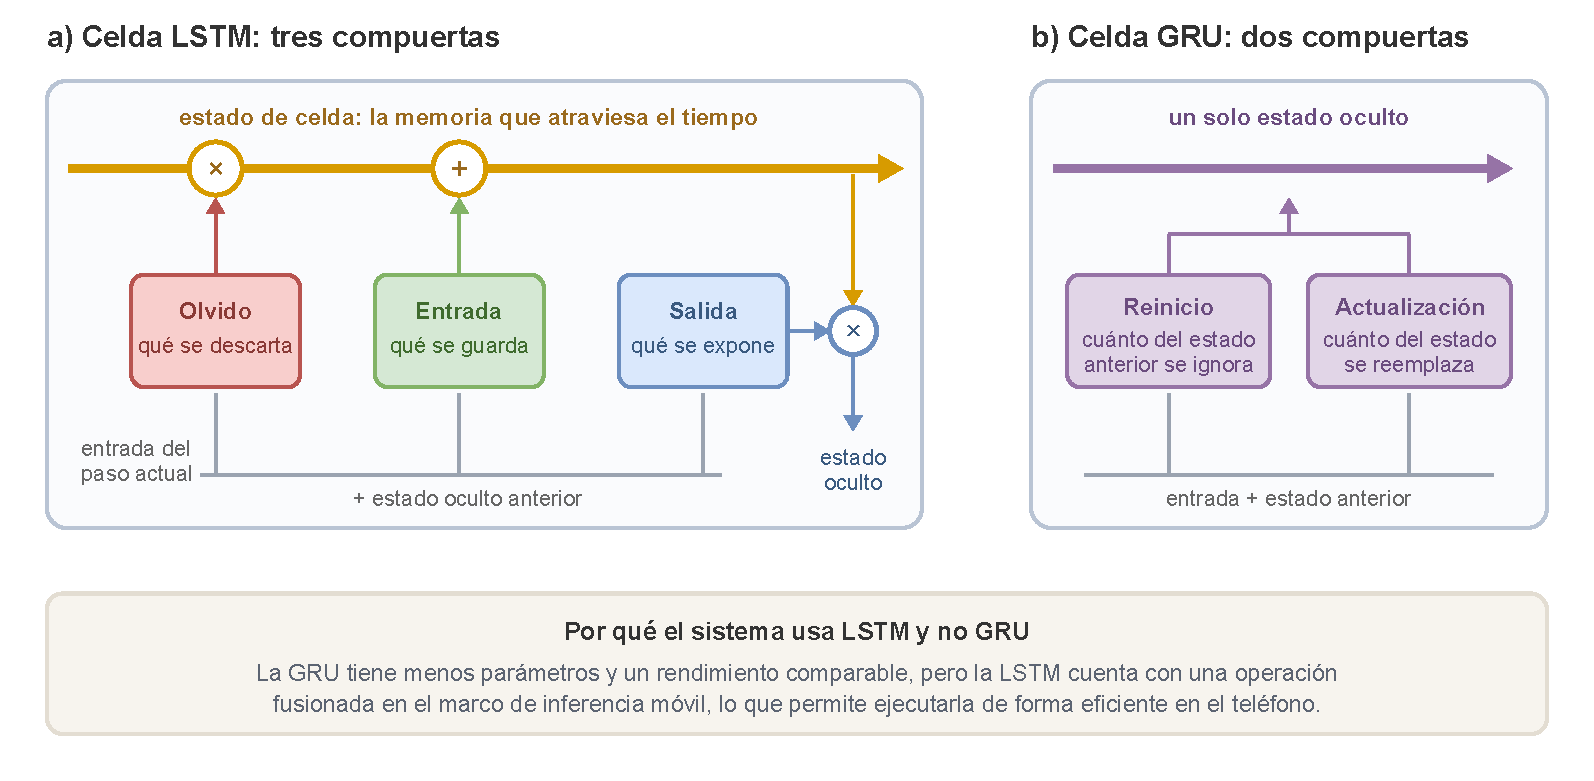
\includegraphics[width=\textwidth]{Figures/Teoria/lstm_gru.pdf}
\caption[Celdas LSTM y GRU]{Esquema simplificado de las celdas \acrshort{lstm} y
\acrshort{gru}. A la izquierda, las tres compuertas de la \acrshort{lstm}: las de olvido y
entrada modifican el estado de celda, que atraviesa la secuencia y funciona como memoria,
mientras que la de salida lo lee para producir el estado oculto. A la derecha, la
\acrshort{gru}, que reduce el mecanismo a dos compuertas sobre un único estado oculto.
Fuente: Elaboración propia.}
\label{fig:teoria-lstm}
\end{figure}

En la \autoref{fig:teoria-lstm} se aprecia por qué la compuerta de olvido resulta
determinante para este
sistema: es la que permite descartar la información de los fotogramas de transición, en
los que la mano viaja entre posiciones sin formar todavía la seña, y conservar en cambio
la del tramo que sí la contiene.

\section{Segmentación Temporal en Flujo Continuo de Gestos}
\label{sec:segmentacion}

En un escenario de uso real, el usuario no realiza señas aisladas frente a la cámara,
sino que produce un flujo continuo de movimientos que incluye señas, transiciones y
movimientos no intencionales. El sistema debe determinar cuándo comienza y cuándo
termina cada seña dentro de este flujo, problema conocido como segmentación temporal,
que representa uno de los desafíos principales del reconocimiento continuo de lengua de
señas \cite{sadik_survey_2025}, \cite{srivastava_continuous_2024}.

El presente sistema adopta una estrategia de segmentación explícita: la persona usuaria
delimita la seña mediante un control en pantalla. Al pulsar el botón de grabación se
activa la captura de la secuencia de landmarks, y al pulsarlo de nuevo la captura se
detiene y la secuencia acumulada se envía al modelo \acrshort{lstm} para su clasificación.
Esta estrategia no requiere modelos adicionales de segmentación ni mecanismos de ventana
deslizante, y funciona con independencia de la duración de la seña.

Durante el desarrollo se evaluó una alternativa que delimitaba la seña con dos gestos de
control reconocidos por el propio modelo del alfabeto, con la intención de que el usuario
no tuviera que tocar la pantalla. Esa alternativa se descartó tras las pruebas en el
dispositivo: varias señas dinámicas del vocabulario juntan las puntas de los dedos con la
mano extendida, una configuración que el modelo confundía con el gesto de cierre, de modo
que la grabación se interrumpía a mitad de la seña. El control explícito en pantalla
resultó más fiable, y el hallazgo se documenta porque delimita una vía que no conviene
seguir sin resolver antes esa ambigüedad.

El deletreo, en cambio, sí opera de forma continua: el modelo del alfabeto clasifica una
ventana tras otra sin que medie ninguna señal de apertura o cierre, de modo que allí el
problema de segmentación persiste. Para evitar clasificaciones inestables causadas por
cuadros de transición, se aplican dos
filtros de postprocesamiento sobre las predicciones del modelo del alfabeto: un filtro de
persistencia temporal que acepta una predicción solo si el modelo produce la misma clase
durante un mínimo de 5 ventanas consecutivas con confianza igual o superior al 60\,\%, y
un período de enfriamiento de 1200 milisegundos tras cada predicción aceptada.

\section{Métricas de Evaluación de Modelos Clasificadores}

Una vez definidas las arquitecturas de los modelos y el mecanismo de segmentación
temporal, es necesario establecer los criterios con los que se medirá su desempeño.

La evaluación de un modelo clasificador parte de la matriz de confusión, una tabla de
$C \times C$ donde $C$ es el número de clases. Cada celda $(i, j)$ contiene el número
de muestras de la clase real $i$ que el modelo clasificó como clase $j$. Los elementos
de la diagonal representan las predicciones correctas, mientras que los elementos fuera
de ella indican errores. Para un sistema de reconocimiento de señas, la matriz de
confusión permite identificar qué señas el modelo confunde con mayor frecuencia,
información especialmente valiosa cuando existen señas visualmente similares
\cite{sokolova_metrics_2009}.

A partir de la matriz de confusión se derivan las métricas estándar. La exactitud
(accuracy) es la proporción de predicciones correctas sobre el total de muestras.
La precisión (precision) de una clase es la proporción de muestras predichas como esa
clase que realmente le pertenecen. La sensibilidad (recall) es la proporción de muestras
de esa clase que el modelo identificó correctamente. La puntuación F1 (F1-score) es la
media armónica de precisión y sensibilidad, útil cuando se busca equilibrar ambas
métricas \cite{sokolova_metrics_2009}. En problemas multiclase con muchas clases, como
los del presente sistema, se utiliza el macro-promedio, que calcula cada métrica de
forma independiente para cada clase y luego promedia los valores, tratando a todas las
clases con igual importancia independientemente de su frecuencia en el conjunto de datos.
Esta elección se justifica porque cada seña de \acrshort{lesho} tiene igual relevancia comunicativa
para el usuario final.

La \autoref{fig:teoria-matriz} muestra un ejemplo con cuatro clases y señala de qué parte
de la matriz se obtiene cada métrica.

\begin{figure}[htbp]
\centering
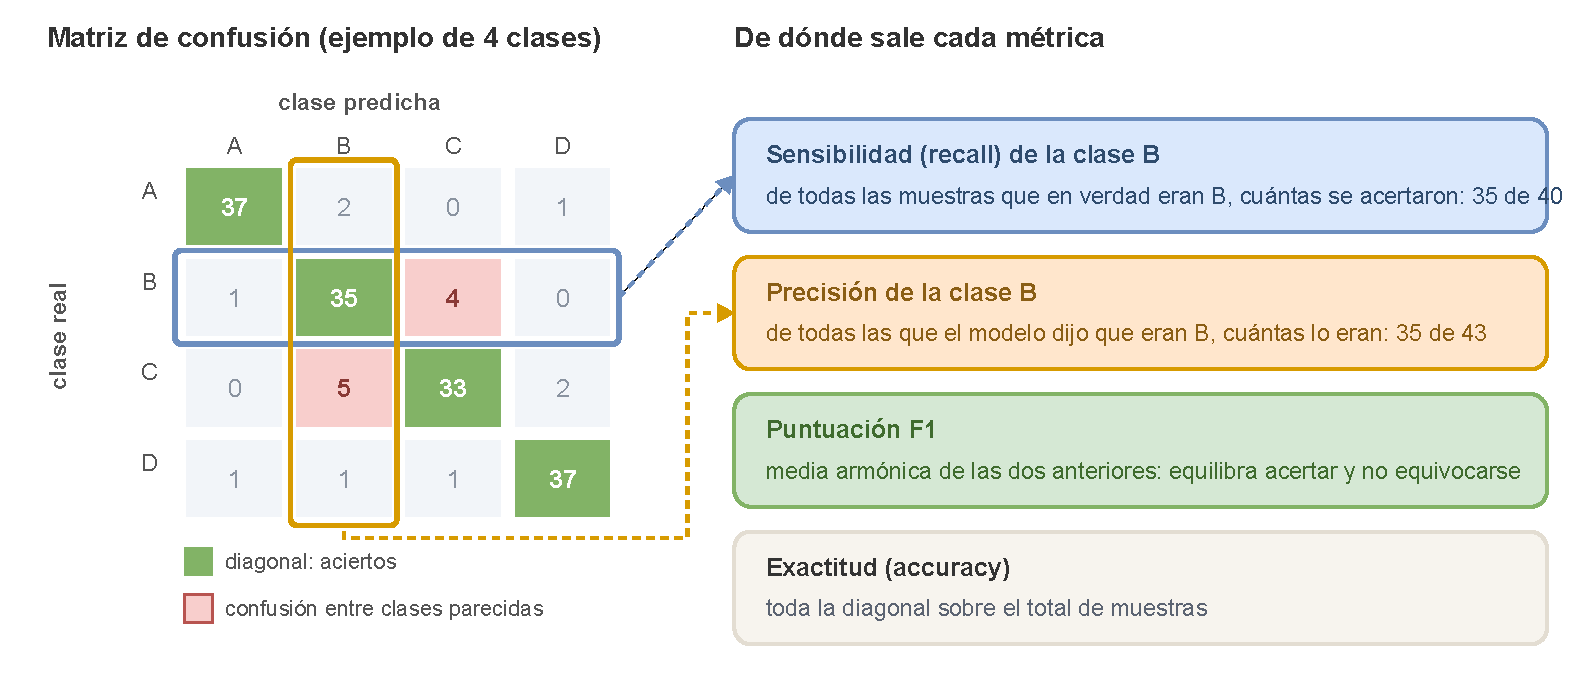
\includegraphics[width=\textwidth]{Figures/Teoria/matriz_confusion.pdf}
\caption[Matriz de confusión y origen de las métricas]{Matriz de confusión de un ejemplo
con cuatro clases. La diagonal concentra los aciertos y las celdas fuera de ella señalan
las confusiones. A la derecha se indica de qué fila o columna se deriva cada métrica.
Fuente: Elaboración propia.}
\label{fig:teoria-matriz}
\end{figure}

La distinción entre la fila y la columna es la que suele prestarse a confusión. La
sensibilidad se lee sobre la fila, porque parte de las muestras que en verdad pertenecen a
la clase; la precisión se lee sobre la columna, porque parte de las que el modelo asignó a
esa clase. Un modelo puede tener sensibilidad alta y precisión baja si acierta casi todas
las muestras de una clase pero además atrae hacia ella muchas de otras.

\section{Inferencia Local en Dispositivos Móviles con TensorFlow Lite}

El diseño del sistema exige que toda la inferencia se ejecute localmente en el teléfono
del usuario, sin enviar datos a un servidor externo. Esta restricción responde a tres
consideraciones: privacidad, disponibilidad en zonas rurales de Honduras sin conexión a
internet, y latencia mínima para que la comunicación sea fluida. TensorFlow Lite (\acrshort{tflite})
es el marco de inferencia de Google diseñado para ejecutar modelos de aprendizaje
automático en dispositivos móviles y con recursos limitados \cite{google_tflite_2024}.
Utiliza un formato de archivo binario basado en FlatBuffer con extensión \texttt{.tflite}
que minimiza el tiempo de carga y la huella de memoria en comparación con el formato
estándar de TensorFlow.

La \autoref{fig:teoria-tflite} resume ese recorrido, desde el modelo entrenado hasta su
ejecución dentro de la aplicación. Los pasos se detallan a continuación.

\begin{figure}[htbp]
\centering
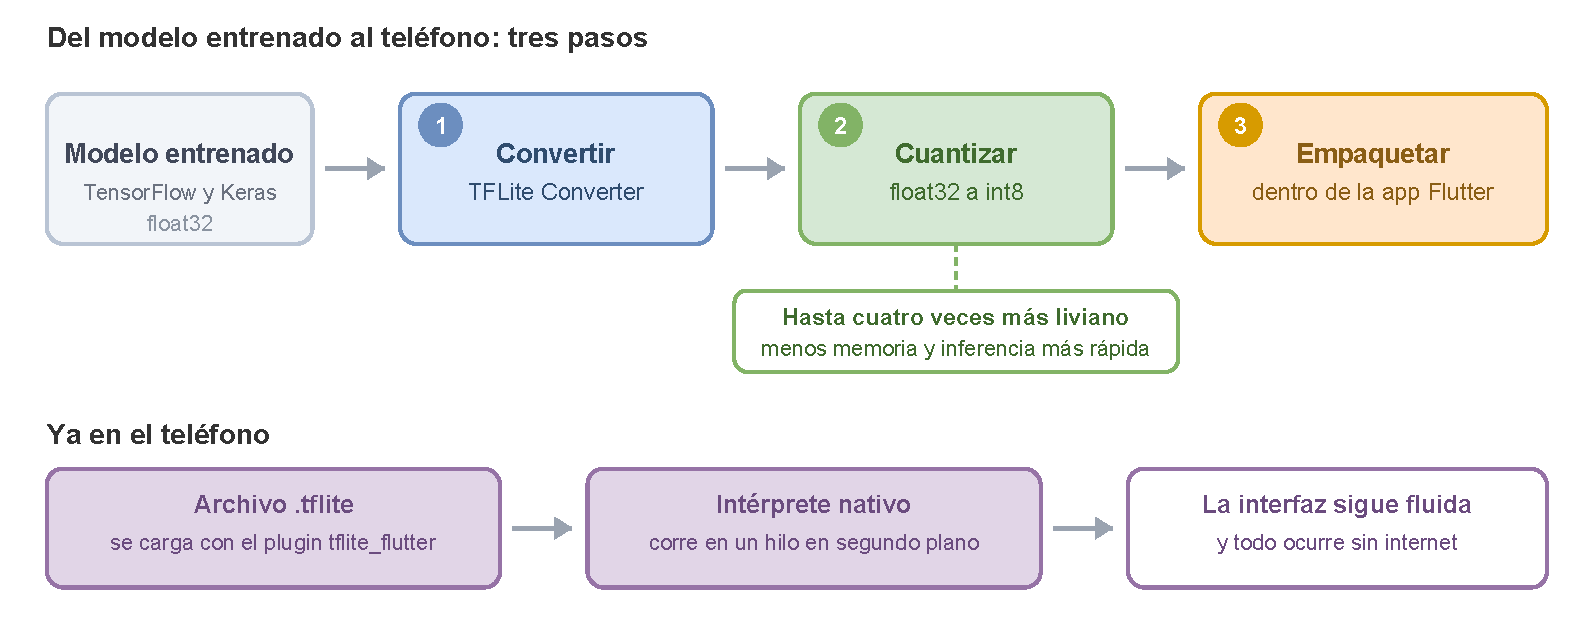
\includegraphics[width=\textwidth]{Figures/Teoria/despliegue_tflite.pdf}
\caption[Flujo de conversión y despliegue con TensorFlow Lite]{Flujo de conversión y
despliegue con \acrshort{tflite}. Arriba, los tres pasos que llevan del modelo entrenado al
archivo empaquetado en la aplicación; abajo, la forma en que ese archivo se carga y se
ejecuta ya en el teléfono. Fuente: Elaboración propia.}
\label{fig:teoria-tflite}
\end{figure}

El flujo de trabajo para desplegar un modelo en el dispositivo consta de tres pasos.
Primero, el modelo entrenado en TensorFlow y Keras se convierte al formato \texttt{.tflite}
mediante el \acrshort{tflite} Converter. Segundo, se aplica cuantización post-entrenamiento para
reducir la precisión numérica de los pesos de punto flotante de 32 bits (float32) a
enteros de 8 bits (int8), lo que reduce el tamaño del modelo hasta cuatro veces,
disminuye el uso de memoria RAM y acelera la inferencia en la CPU del dispositivo
\cite{google_tflite_2024}, \cite{google_quantization_2024}. Tercero, el archivo
\texttt{.tflite} se empaqueta dentro de la aplicación Flutter y se carga mediante el
plugin \texttt{tflite\_flutter}, que proporciona una interfaz en Dart para el intérprete
nativo de \acrshort{tflite} a través de \acrshort{ffi} (Foreign Function Interface). El procesamiento de los cuadros de video se
ejecuta en un hilo nativo en segundo plano, comunicado con la aplicación mediante un canal
de plataforma, lo que garantiza que la interfaz responda con fluidez durante la ejecución
del sistema.
El \autoref{ch:implementacion} detalla la configuración específica de los modelos dentro
de la aplicación, y el \autoref{chap:resultados} reporta el tamaño final de los archivos
convertidos y los tiempos de inferencia medidos en el dispositivo de prueba.

El paso de cuantización es el que hace viable el despliegue en un dispositivo de gama
baja: al reducir la precisión numérica de los pesos, el archivo se aligera de forma
notable y la inferencia se acelera, a cambio de una pérdida de exactitud que en la
práctica resulta mínima para tareas de clasificación como esta.
